% This template has been tested with LLNCS DOCUMENT CLASS -- version 2.20 (24-JUN-2015)

%"runningheads" enables:
%  - page number on page 2 onwards
%  - title/authors on even/odd pages
%This is good for other readers to enable proper archiving among other papers and pointing to
%content. Even if the title page states the title, when printed and stored in a folder, when
%blindly opening the folder, one could hit not the title page, but an arbitrary page. Therefore,
%it is good to have title printed on the pages, too.
\documentclass[runningheads,a4paper]{llncs}[2015/06/24]

%cmap has to be loaded before any font package (such as cfr-lm)
\usepackage{cmap}
\usepackage[T1]{fontenc}

\usepackage{graphicx}

% für neue deutsche Rechtschreibung
%\usepackage[english,ngerman]{babel}

% für englische Rechtschreibung
%Even though `american`, `english` and `USenglish` are synonyms for babel package (according to https://tex.stackexchange.com/questions/12775/babel-english-american-usenglish), the llncs document class is prepared to avoid the overriding of certain names (such as "Abstract." -> "Abstract" or "Fig." -> "Figure") when using `english`, but not when using the other 2.
%english has to go last to set it as default language
\usepackage[ngerman,english]{babel}

%Eingabeformat UTF-8
\usepackage[utf8]{inputenc}

%Hint by http://tex.stackexchange.com/a/321066/9075 -> enable "= as dashes
\addto\extrasenglish{\languageshorthands{ngerman}\useshorthands{"}}

%cfr-lm is preferred over lmodern. Reasoning at http://tex.stackexchange.com/a/247543/9075
\usepackage[%
rm={oldstyle=false,proportional=true},%
sf={oldstyle=false,proportional=true},%
tt={oldstyle=false,proportional=true,variable=true},%
qt=false%
]{cfr-lm}
%
%if more space is needed, exchange cfr-lm by mathptmx

\graphicspath{{graphics/}}

%Tweaks by IPVS/AS
\usepackage{lncs_as}

%for demonstration purposes only
\usepackage[math]{blindtext}

%Sorts the citations in the brackets
%It also allows \cite{refa, refb}. Otherwise, the document does not compile.
%  Error message: "White space in argument"
\usepackage{cite}


%% If you need packages for other papers,
%% START COPYING HERE
%% COPY ALSO cmap and fontenc from lines 10 to 12

%extended enumerate, such as \begin{compactenum}
\usepackage{paralist}

%put figures inside a text
%\usepackage{picins}
%use
%\piccaptioninside
%\piccaption{...}
%\parpic[r]{\includegraphics ...}
%Text...

%for easy quotations: \enquote{text}
\usepackage{csquotes}

%enable margin kerning
\usepackage{microtype}

%tweak \url{...}
\usepackage{url}
%\urlstyle{same}
%improve wrapping of URLs - hint by http://tex.stackexchange.com/a/10419/9075
\makeatletter
\g@addto@macro{\UrlBreaks}{\UrlOrds}
\makeatother
%nicer // - solution by http://tex.stackexchange.com/a/98470/9075
%DO NOT ACTIVATE -> prevents line breaks
%\makeatletter
%\def\Url@twoslashes{\mathchar`\/\@ifnextchar/{\kern-.2em}{}}
%\g@addto@macro\UrlSpecials{\do\/{\Url@twoslashes}}
%\makeatother

%diagonal lines in a table - http://tex.stackexchange.com/questions/17745/diagonal-lines-in-table-cell
%slashbox is not available in texlive (due to licensing) and also gives bad results. This, we use diagbox
%\usepackage{diagbox}

%required for pdfcomment later
\usepackage[hyperref,svgnames]{xcolor}

\usepackage{listings}
\lstloadlanguages{java}
\lstset{language=java,numbers=left,captionpos=b}


%enable nice comments
%this also loads hyperref
\usepackage{pdfcomment}
%enable hyperref without colors and without bookmarks
\hypersetup{hidelinks,
   colorlinks=true,
   allcolors=black,
   pdfstartview=Fit,
   breaklinks=true}
%enables correct jumping to figures when referencing
\usepackage[all]{hypcap}

\newcommand{\commentontext}[2]{\colorbox{yellow!60}{#1}\pdfcomment[color={0.234 0.867 0.211},hoffset=-6pt,voffset=10pt,opacity=0.5]{#2}}
\newcommand{\commentatside}[1]{\pdfcomment[color={0.045 0.278 0.643},icon=Note]{#1}}

%compatibality with packages todo, easy-todo, todonotes
\newcommand{\todo}[1]{\commentatside{#1}}
%compatiblity with package fixmetodonotes
\newcommand{\TODO}[1]{\commentatside{#1}}

%enable \cref{...} and \Cref{...} instead of \ref: Type of reference included in the link

%\usepackage[capitalise,nameinlink,ngerman]{cleveref}
\usepackage[capitalise,nameinlink,english]{cleveref}
%Nice formats for \cref - only for English texts
%\crefname{section}{Sect.}{Sect.}
%\Crefname{section}{Section}{Sections}

\usepackage{xspace}
%\newcommand{\eg}{e.\,g.\xspace}
%\newcommand{\ie}{i.\,e.\xspace}
\newcommand{\eg}{e.\,g.,\ }
\newcommand{\ie}{i.\,e.,\ }

%introduce \powerset - hint by http://matheplanet.com/matheplanet/nuke/html/viewtopic.php?topic=136492&post_id=997377
\DeclareFontFamily{U}{MnSymbolC}{}
\DeclareSymbolFont{MnSyC}{U}{MnSymbolC}{m}{n}
\DeclareFontShape{U}{MnSymbolC}{m}{n}{
    <-6>  MnSymbolC5
   <6-7>  MnSymbolC6
   <7-8>  MnSymbolC7
   <8-9>  MnSymbolC8
   <9-10> MnSymbolC9
  <10-12> MnSymbolC10
  <12->   MnSymbolC12%
}{}
\DeclareMathSymbol{\powerset}{\mathord}{MnSyC}{180}

% correct bad hyphenation here
\hyphenation{op-tical net-works semi-conduc-tor}

%% END COPYING HERE


\begin{document}

\title{Apache Storm}
%If Title is too long, use \titlerunning
%\titlerunning{Short Title}

\author{Aanal Raj Basaula}

\supervisor{Matthias Wieland}

\seminar{Seminarbezeichung}

\semester{WS 2017/2018}

\abgabedatum{Stuttgart, 11.12.2017}

\institute{\email{aanal.basaula@gmail.com}}

%\frontpagede % creates the frontpage (in German)
\frontpageen % creates the frontpage (in English)

\thispagestyle{empty}
\cleardoublepage

\maketitle

\begin{abstract}
In today's world everyone is connected to this ever increasing network of computers be it via a Personal computer, a smart phone or an Embedded Device such as your smart home appliances. These devices generate a huge amounts of data every instance, that can be analyzed to leverage business opportunities previously undiscovered. To be able to discern these windows of opportunities, one must be able to process and analyze the data. In this report we talk about such scenario and the available tools which allows us to process large data streams with minimum latency.
\end{abstract}

\begin{keywords}
Apache Storm, Stream Processing, Real Time Processing, Big Data
\end{keywords}

\section{Introduction}

\textbf{Data} today is generated by a lot of devices that are connected to the internet and the amount of data being generated at any instance is increasing rapidly. The above mentioned device could be a Personal Computer, a Smart phone, or even an Embedded System. Due to the rapid adoption of Internet of Things, data is being generated at a rate that is unprecedented. The sheer volume of data generated and at the rate at which it is being generated can be termed as Big Data. \textbf{Big Data} made it's appearance in 1998 SGI slide by John Mashey and now is of interest to a lot of financial as well as research institutions.[1]

Data can be considered the oil of the current age, because with huge amounts of data one can determine hidden patterns. A lot of companies utilize pattern recognition on big data to open opportunities for revenue generation whereas research institutions use it to discover something new. The question on how to classify any data as big data can be answered by using the 3Vs of big data: Volume, Variety and Velocity [2]. Any data with big volume or variety (such as text, video, images, etc) or that gets generated rapidly can be considered as big data. In this paper regarding \textbf{Apache Storm} we consider the third V of big data to be the influencing factor.

\textbf{Data Stream} is a sequence of data flowing from a source to a destination, for example a sensor reporting the temperature to a server. The sensor measures the temperature periodically and updates it to the server. Another example could also be the purchase requests of your product. In all of these scenarios, the data is continuously being generated. Traditionally analyzing of these types of data requires storage of these data onto persistence and later batch processing it to discern patterns as well as other useful information. But, with the help of \textbf{Apache Storm} we are able to process these data as they are generated with minimum amount of latency.

This benefit could be a major game changer for many companies as Stream processing of data allows Real Time Analysis. As an example, an online store could monitor its purchase requests for best performing and least performing articles and could offer discounts on the articles not performing good to increase their sales volume. This small change could increase the earnings of a company and will surely be advantageous.

\section{Apache Storm: Concepts}

Apache storm is one of the available open source tools for stream data processing, which is considered to be one of the most easy to use, fast and fault tolerant systems available [3]. These three factors have been the major points for the general public to choose \textbf{Apache Storm} above other available tools. It was originally created by Nathan Marz at BackType and till now, at present more than 60 companies use or experiment with this tool.

\subsection{Architecture}
The basic Storm data processing architecture consists of stream of tuples flowing through a defined topology to yield the required analytic result. Processing of this stream data is performed in Nodes called the worker nodes, which are responsible for performing the required calculations. There is also another node named the Master Node, which is responsible for the complete Storm infrastructure,  by keeping track of all the worker nodes and the total topology itself.

\begin{figure}
  \begin{center}
    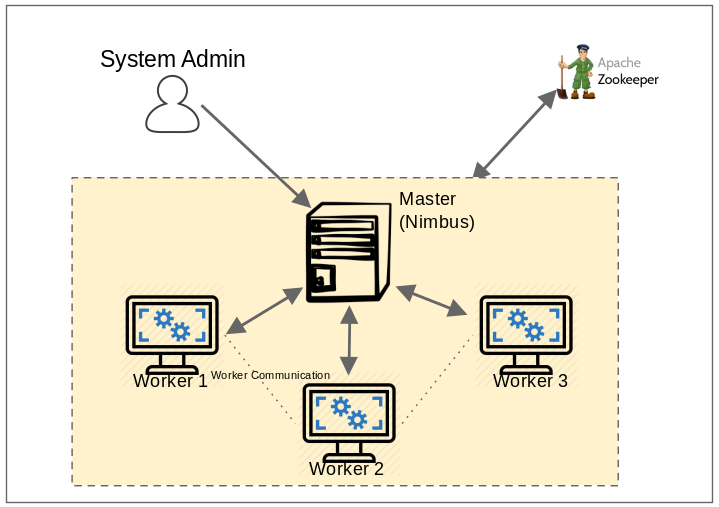
\includegraphics[width=.5\textwidth]{arch.png}
    \caption{High Level Storm Architecture}
    \label{fig:arch}
   \end{center}
\end{figure}

\subsubsection{Nimbus}

\paragraph{The Master node} also called the \textbf{Nimbus} is also responsible for distribution and coordination of the execution of topologies. The Nimbus is the first point where the user submits the defined topology, which is then distributed among the worker nodes.  Figure \ref{fig:arch} illustrates the high level architecture where, Nimbus monitors all the available worker nodes and both the nimbus as well as the worker nodes use \textbf{Apache Zookeeper} to store their states. The actual processing is done by the \textbf{worker nodes}, and each worker node runs multiple Worker Processes each of them mapped to their own topology [4]. It is also worth while noting that multiple worker processes in a worker node could be executing different parts of the topology.

\subsubsection{Worker Node}
\paragraph{Worker Node} is responsible for all the heavy lifting required for processing of the topology. One worker node may run a multiple number of worker processes. Each of these worker processes may belong to the same topology or different topologies. A worker node maintains a \textbf{Supervisor} and a multiple number of Worker Processes which in turn maintains a multiple number of executors. Thus, Executors enable intra-topology parallelism whereas Tasks provide intra-spout or intra-bolt parallelism. Figure \ref{fig:workerarch} depicts the design of a Worker node.[4]

\begin{figure}
  \begin{center}
    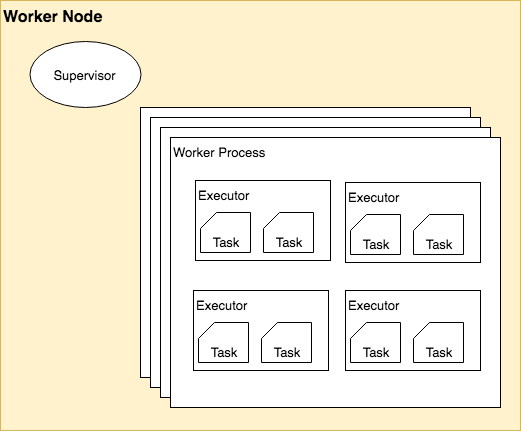
\includegraphics[width=.5\textwidth]{worker.png}
    \caption{Worker Node Architecture}
    \label{fig:workerarch}
   \end{center}
\end{figure}

\paragraph{Supervisor} is running in every Worker Node and communicates with the Nimbus to receive assignments from it. Apart from taking assignments from the Nimbus it is also responsible for monitoring the health of the of the worker processes and respawns the worker processes in case it dies.

\paragraph{Worker Process} is the Entity that does the processing and is mapped to a certain topology. Each worker node spawns a JVM and runs one or multiple executors. These executors may be running any of the bolt or spout within the topology, thus providing an added level of parallelism.

\paragraph{Executors} are made up of one or multiple Tasks. Unless specified explicitly, storm assigns single task to a single executor. Executors takes tuples from the in queue, examines the task this tuple is destined to, performs the task and then places the result in the out queue [4].

\subsection{Topology}
\paragraph{Topology} is a directed graph where the vertices represent computation and the edges represents the data flow. Another important thing about topologies in Storm is that they are allowed to have cycles. Figure \ref{fig:topo} shows a basic Storm Topology, which consists of Spouts and Bolts. Spouts are the Sources of tuples in a Topology whereas Bolts are the units which process these generated tuples. The user first submits the topology to the Apache Storm Nimbus, which consults with each of the available Supervisors in the worker nodes and assigns each of them with tasks related to the topology.

\begin{figure}
  \begin{center}
    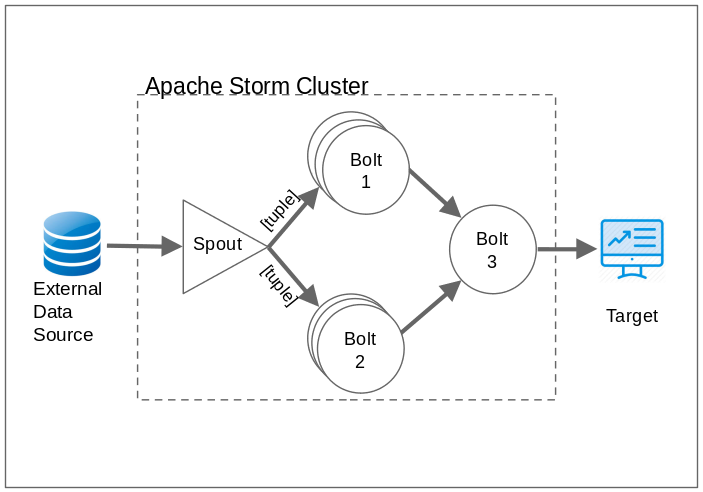
\includegraphics[width=.7\textwidth]{topo.png}
    \caption{Generic Storm Topology}
    \label{fig:topo}
   \end{center}
\end{figure}

\subsubsection{Spout} is the entry point for any data in the Storm Topology. As shown in the figure \ref{fig:topo} spouts take data from external source and emits them into the topology as tuples. The input source could be a Heterogenous data source.

\subsubsection{Bolt} are the processing entities of a Topology. It receives raw tuples emitted by spouts or processed tuples sent by another bolt and sends it down the pipe after it has completed its processing.

\section{Practical Use Case}
Apache Storm is used for stream processing of data, in many sources [2,3] a word frequency count example has been shown which can be considered to be trivial, but in actual practice it can be used to execute complicated algorithms. For the purposes of this paper we consider a trivial but different example of \textbf{Sentiment Analysis}.

\subsection{Scenario}

\subsubsection{Description}
\paragraph{Let us consider} a company which produces a range of products, for example \textbf{Apple Inc.} produces IPhones, IPods, MacBooks, etc. For such a big company an understanding of the sentiment of the people is important to maintain a positive outlook. The company can also analyze the feedback people place on a specific product, to change and adjust the pricing schemes in real time to the demand.  At present there are many social media networks available and people tend to share their views on these networks,  \textbf{Twitter} is also one of these social networks where a number of posts are available publicly and can be analyzed to obtain a generalized view about a specific product or the company in general.

\subsubsection{Proposed Solution}

\paragraph{Solution} to the scenario can be implemented using \textbf{Apache Storm} to process the tweets in real time. Figure \ref{fig:solution} shows the simplified system overview, consisting of Twitter Streaming Servers as the source of information. This information is processed in the Storm Clusters from within the Company Infrastructure and the analyzed result is reported to the User Interface, which can be accessed by the appropriate user.

\begin{figure}
  \begin{center}
    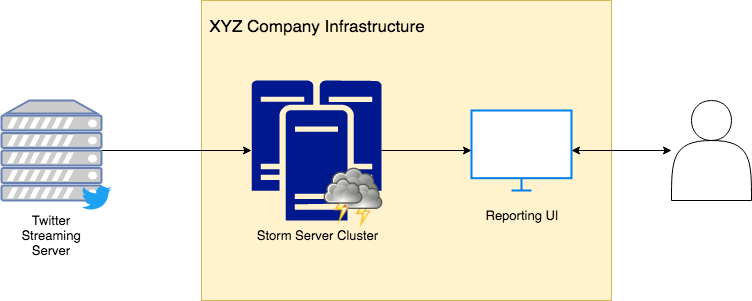
\includegraphics[width=.7\textwidth]{solution.png}
    \caption{Generic Streaming Solution implemented in this use case}
    \label{fig:solution}
   \end{center}
\end{figure}

\paragraph{This} is not the only possible solution, there are multiple other tools such as \textbf{Spark Streaming}, \textbf{Samza}, etc. but this paper considers Apache Storm as it is in the spotlight of this paper, for further details regarding other available tools and their comparisons with Apache Storm, please consider the section \ref{sec:othertools} for further details.

\subsection{Practical Implementation}

\section{Other Tools}
 \label{sec:othertools}

\section{Einleitung}
Ab diesem Abschnitt fängt die eigentliche Arbeit an und man beginnt mit einer Einführung und der Einordnung des Themas.

Absätze werden durch Leerzeilen erreicht.

Als \LaTeX-Editor sind TeXstudio\footnote{\url{http://texstudio.sourceforge.net/}} oder TeXlipse\footnote{\url{http://texlipse.sourceforge.net/}} empfehlenswert.

Für die Versionskontrolle bietet es sich an, jeden Satz in einer neuen Zeile zu beginnen.

Als Nachschlagewerk und gute Einführung in das Thema \LaTeX\ bietet sich \emph{The Not So Short Introduction to \LaTeXe}\ von Oetiker et al an.
Auf der Seite \url{http://tobi.oetiker.ch/lshort/} ist dieses Dokument zum Herunterladen bereitgestellt.

Ein weiteres, empfehlenswertes Dokument ist das \emph{Kochbuch für \LaTeX{}}, welches auf der Seite \url{http://www.uni-giessen.de/hrz/tex/cookbook/cookbook.html} zu finden ist.

Eine Vorlage für Bachelor- und Masterarbeiten ist unter \url{https://github.com/latextemplates/uni-stuttgart-computer-science-template} zu finden.

Für weitere Anleitungen und Informationen empfiehlt sich die Homepage \url{http://www.dante.de/}.
Des Weiteren gibt es eine Reihe von Literatur zum Thema \LaTeX\ von Bürger~\cite{buerger}, Kopka~\cite{kopka}, Günther~\cite{guenther} und vielen anderen.
Weitere Hinweise zu \LaTeX{} unter \url{http://wiki.flupp.de/latex}.
Zu Ausarbeitungen im Allgemeinen unter \url{http://wiki.flupp.de/studium/ausarbeitungen}.

Die Arbeit gleidert sich wie folgt:
...
Schließlich wird in \cref{sec:zusfas} eine Zusammenfassung der Arbeit und ein Ausblick auf weitere Forschungsthemen gegeben.

\subsection{Beispiel für Überschrift 2.~Ebene}

\subsubsection{Beispiel für Überschrift 3.~Ebene}

\paragraph{Beispiel für Überschrift 4.~Ebene}
Dies ist Beispielabsatz zu einem Beispiel einer Überschrift 4.~Ebene.

\section{Formatierungsrichtlinien}

\subsection{Tabellen}
In diesem Abschnitt wird das Einfügen einer Tabelle und das Füllen derselben mit Werten gezeigt.
Im Gegensatz zu Abbildungen erfolgt die Beschriftung üblicherweise oberhalb und nicht unterhalb der Tabelle.
Der letzte Satz der Beschriftung endet ohne Punkt.
Die \Cref{tab:bsp} zeigt die Größenentwicklung der Weltbevölkerung von 8000 v.\,Chr. bis 1980 n.\,Chr.

\begin{table}
\caption{Dieses Beispiel entstammt dem {\it\TeX{}Buch,} S.\,246}
\label{tab:bsp}
\begin{center}
\begin{tabular}{r@{\quad}rl}
\hline
\multicolumn{1}{l}{\rule{0pt}{12pt}
                   Jahr}&\multicolumn{2}{l}{Weltbevölkerung}\\[2pt]
\hline\rule{0pt}{12pt}
8000 v.\,Chr. &     5,000,000& \\
  50 n\,Chr. &   200,000,000& \\
1650 n\,Chr. &   500,000,000& \\
1945 n\,Chr. & 2,300,000,000& \\
1980 n\,Chr. & 4,400,000,000& \\[2pt]
\hline
\end{tabular}
\end{center}
\end{table}

\subsection{Code-Beispiele}

\Cref{lst:example} zeigt ein Code-Beispiel.

\begin{lstlisting}[float,caption=A floating example,label=lst:example]
public static void main(String[] args) {
}
\end{lstlisting}

\subsection{Formeln}
Formeln sind in aufsteigender Reihenfolge, beginnend mit der Nummer~1, durchzunummerieren.
Dies erleichtert den Bezug vom Text auf die zugehörige Formel.
Die Formel
%
\begin{equation}
  \psi (u) = \int_{o}^{T} \left[\frac{1}{2}
  \left(\Lambda_{o}^{-1} u,u\right) + N^{\ast} (-u)\right] dt
\end{equation}
%
berechnet etwas.
Formeln sind bezüglich der Zeichensetzung wie normaler Text zu behandeln, d.\,h.\ falls ein Satz mit einer Formel endet, folgt dieser ein Punkt, der üblicherweise durch ein schmales Leerzeichen abgesetzt wird.

\subsection{Abbildungen}
Im nachfolgenden Beispiel wird dargestellt, wie Grafiken eingefügt werden und wie die Beschriftung bzw.\ die Formatierung derselben auszusehen hat.

Bei Abbildungen erfolgt die Beschriftung unterhalb der Abbildung (siehe \cref{fig:logo}).
Der letzte Satz der Beschreibung endet wie bei Tabellenbeschriftungen ohne Punkt.
Um eine gute Qualität zu erzielen, muss die Auflösung der Abbildungen mindestens 300~DPI betragen.
Bei Strichzeichnungen empfiehlt sich sogar eine weit höhere Auflösung, zwischen 800 und
1200~DPI.

Am besten Vektorgraphiken nehmen und als \texttt{.pdf} exportieren.

\begin{figure}
  \begin{center}
    
\includegraphics[width=.5\textwidth]{ipvslogo.png}
    \caption{Das Logo des Instituts}
    \label{fig:logo}
   \end{center}
\end{figure}

\subsection{Literaturverweise}
Ein Verweis auf eine im Literaturverzeichnis aufgeführte
Literaturquelle wird durch die in eckige Klammern eingeschlossene
Nummer der entsprechenden Literaturquelle angegeben. Als Beispiel ist
hier nochmals auf Buerger~\cite{buerger} verwiesen.

\subsection{Anführungszeichen}
Entweder "`so"' tippen oder \enquote{so}.
``So'' bitte nicht, das führt zu englischen Anführungszeichen.

\subsection{Sonstiges}
Brackets work as designed:
<test>

The symbol for powerset is now correct: $\powerset$ and not a Weierstrass p ($\wp$).

\begin{inparaenum}
\item All these items...
\item ...appear in one line
\item This is enabled by the paralist package.
\end{inparaenum}

``something in quotes'' using plain tex or use \enquote{the enquote command}.

You can now write words containing hyphens which are hyphenated (application"=specific) at other places.
This is enabled by an additional configuration of the babel package.
In case you write \enquote{application-specific}, then the word will only be hyphenated at the dash.
You can also write applica\allowbreak{}tion-specific, but this is much more effort.

\section{Zusammenfassung}
\label{sec:zusfas}
Dieser Absatz schließt die Arbeit ab.

\subsubsection*{Acknowledgments}
...

In the bibliography, use \texttt{\textbackslash textsuperscript} for ``st'', ``nd'', ...:
E.g., \enquote{The 2\textsuperscript{nd} conference on examples}.
When you use \href{https://www.jabref.org}{JabRef}, you can use the clean up command to achieve that.
See \url{https://help.jabref.org/en/CleanupEntries} for an overview of the cleanup functionality.

%%%%%%%%%%%%%%%%%%%%%%%%%%%%%%%%%%%%%%%%%%%%%%%%%%%%%%%%%%%%%%%%%%%%%%%%%%%%%%%

\bibliographystyle{splncs03}
\bibliography{paper}
Alle Links wurden zuletzt am 22.06.2015 geprüft.
\end{document}
